\documentclass[11pt,a4paper]{article}
\usepackage[margin=2.5cm]{geometry}
\usepackage{amsmath,amssymb,booktabs,graphicx,xcolor,hyperref,microtype}
\usepackage{authblk}
\hypersetup{colorlinks=true,linkcolor=blue,citecolor=blue,urlcolor=blue}

\newcommand{\Corder}{C_{\mathrm{order}}}
\newcommand{\sw}{\sigma_w}
\newcommand{\na}{\mathrm{na\_ratio}}
\newcommand{\Pcausal}{P_{\mathrm{causal}}}
\newcommand{\Psp}{P_{\mathrm{spatial}}}
\newcommand{\Ptemp}{P_{\mathrm{temporal}}}
\newcommand{\Phist}{P_{\mathrm{hist}}}
\newcommand{\Lf}{\mathcal{L}}

\title{\textbf{Paper 59: Field Equation of VCML, Historical Causal Purity,\\
and the Structural Origin of the $r_\mathrm{wave}=8$ Anomaly}\\
\large From Discrete Update Rules to a Model A Field Theory}

\author[1]{Gabriel Aubin-Moreau}
\affil[1]{Independent research}
\date{March 2026}

\begin{document}
\maketitle

\begin{abstract}
Paper~58 reduced the identity condition to two causal purity dimensions
($\Psp$ and $\Ptemp$) but left one anomaly unexplained:
$r_\mathrm{wave}=8$ fails for C\_perturb despite $\Psp=0.905$
and $\Ptemp=1$.
We investigate whether a third dimension---\emph{historical purity}
$\Phist$ (fraction of mid\_mem content at consolidation originating
from same-zone waves)---closes this gap.

\textbf{Finding 1 (null result):}
Empirical $\Phist \approx \Psp$ across all conditions (within 0.001--0.038).
The geometric prediction for $\Phist$ is a severe underestimate (0.68--0.84 predicted
vs.\ 0.93--0.98 measured), corrected by the same launch-area asymmetry identified in
Paper~57.
Historical purity is \emph{not} a distinct third dimension.

\textbf{Finding 2 (from the null result):}
The two-purity framework of Paper~58 is sufficient: $\Psp$ and $\Ptemp$ are
sufficient statistics for the noise injected into fieldM. The mid\_mem accumulation
does not independently contaminate the causal signal beyond what a single-event
measurement captures.

\textbf{Finding 3 (structural):}
We derive the continuous-time field equation of VCML.
fieldM obeys a \emph{Model~A} (stochastic relaxation) equation with three noise
channels corresponding to $1-\Psp$, $1-\Ptemp$, and substrate noise.
$\Corder$ is the ratio of the order-parameter amplitude to the fluctuation
amplitude in this field theory---the standard non-equilibrium signal-to-noise ratio.

\textbf{Finding 4 (r\_{wave}=8 characterization):}
The field equation at $r_\mathrm{wave}\approx W_\mathrm{zone}/2.5$
enters a \emph{parity-resonance} regime: waves of this radius transfer the
excitatory/inhibitory zone coloring most efficiently to adjacent zones,
causing fieldM to encode the suppress/excite parity (zones 0,2 vs.\ zones 1,3)
rather than spatial position.
This inverts the na\_ratio signature, making D\_adj $>$ D\_nonadj (na~$<1$).
The anomaly is a structural failure in the drive pattern, not a causal purity failure.
\end{abstract}

%──────────────────────────────────────────────────────────────────────────────
\section{Introduction}

Papers~57--58 established the two-dimensional causal purity condition:
\begin{equation}
  \dot{\Corder} > 0 \iff \Psp > p_c^\mathrm{sp}
  \;\text{ AND }\; \Ptemp > p_c^\mathrm{temp}.
  \label{eq:2d}
\end{equation}
One anomaly remained: C\_perturb at $r_\mathrm{wave}=8$ has $\Psp=0.905$ and
$\Ptemp=1$, yet fails ($\na=0.943$).
Both purity conditions are satisfied but identity does not form.

Three hypotheses:
\begin{enumerate}
  \item \textbf{Historical purity $\Phist$}: mid\_mem at consolidation contains
    contamination from \emph{all prior} waves, not just the triggering one.
    Even with $\Ptemp=1$ and $\Psp\approx 1$ per event, the accumulated
    mid\_mem may be contaminated.
  \item \textbf{Field equation structural change}: at $r_\mathrm{wave}\approx W_\mathrm{zone}/2$,
    the effective drive pattern changes character, encoding zone polarity rather
    than zone location.
  \item \textbf{Minimum copy-forward rate}: the signal growth term in the
    Lyapunov condition may be insufficient at this $\delta$.
\end{enumerate}

We measure $\Phist$ empirically (Hypothesis~1), derive the field equation
(Hypothesis~2), and analyze the drive pattern at $r_\mathrm{wave}=8$.

%──────────────────────────────────────────────────────────────────────────────
\section{Historical Causal Purity: Definition and Measurement}

\paragraph{Definition.}
For each cell $i$, define the exponentially weighted contamination of mid\_mem
at time $t$:
\begin{align}
  M^\mathrm{pure}(i,t) &= \sum_{\tau \leq t} \text{MID\_DECAY}^{t-\tau}
    \cdot \mathrm{FA} \cdot \|dev_i(\tau)\| \cdot
    \mathbf{1}[z_\mathrm{wave}(\tau,i) = z_i] \\
  M^\mathrm{total}(i,t) &= \sum_{\tau \leq t} \text{MID\_DECAY}^{t-\tau}
    \cdot \mathrm{FA} \cdot \|dev_i(\tau)\| \cdot
    \mathbf{1}[w_a(\tau,i) > 0]
\end{align}
where both sums accumulate only during active wave contact ($w_a > 0$).
The historical purity at consolidation time $t$ for cell $i$ is:
\begin{equation}
  \Phist(i,t) = M^\mathrm{pure}(i,t) / M^\mathrm{total}(i,t).
\end{equation}
The aggregate $\Phist$ is the mean over all consolidation events.

\paragraph{Geometric prediction.}
By the same zone-launch area argument as Paper~57:
\begin{equation}
  \Phist^\mathrm{geom}(\delta) = \frac{1}{W_\mathrm{zone}}
  \sum_{x=1}^{W_\mathrm{zone}-1}
  \frac{W_\mathrm{zone}}{W_\mathrm{zone} + 2\min(x,\,W_\mathrm{zone}-x,\,r_\mathrm{wave})}.
\end{equation}
This predicts $\Phist = 0.84$ at $r_\mathrm{wave}=2$ and $\Phist=0.68$ at $r_\mathrm{wave}=8$
--- substantially lower than $\Psp$.

%──────────────────────────────────────────────────────────────────────────────
\section{Results: P\_hist Is Not a Third Dimension}

\begin{table}[h]
\centering
\caption{Empirical $\Psp$, $\Phist$, geometric $\Phist$ prediction, $\sw$, and na at step~3000.
Mean over 5 seeds.}
\label{tab:main}
\begin{tabular}{llrrrrr}
\toprule
Mode & $r$ & $\Psp$ & $\Phist$ (emp.) & $\Phist$ (geom.) & $\sw$ & na \\
\midrule
CP  & 2  & 0.981 & 0.982 & 0.841 & 0.0111 & 1.261 \\
CP  & 4  & 0.948 & 0.955 & 0.753 & 0.0452 & 1.140 \\
CP  & 8  & 0.905 & 0.943 & 0.684 & 0.0961 & 0.943 \\
CP  & 10 & 0.883 & 0.931 & 0.678 & 0.1060 & 1.091 \\
\midrule
ref & 2  & 0.984 & 0.984 & 0.841 & 0.1630 & 1.001 \\
ref & 4  & 0.956 & 0.958 & 0.753 & 0.2277 & 1.081 \\
ref & 8  & 0.928 & 0.944 & 0.684 & 0.1805 & 0.941 \\
ref & 10 & 0.906 & 0.932 & 0.678 & 0.1542 & 1.047 \\
\bottomrule
\end{tabular}
\end{table}

\subsection{Finding 1: Empirical P\_hist $\approx$ P\_sp}

Across all 8 conditions, $|\Phist - \Psp| \leq 0.04$.
At $r=2$: $(0.982, 0.981)$; at $r=8$: $(0.943, 0.905)$; at $r=10$: $(0.931, 0.883)$.
The discrepancy is small and goes in the direction of $\Phist > \Psp$
(mid\_mem history is \emph{more} pure than the single-event measurement, not less).

The geometric prediction is severely wrong: it predicts $\Phist = 0.684$ at $r=8$
but we measure $0.943$.
The same zone-launch area asymmetry identified in Paper~57 applies:
the mid\_mem accumulation is dominated by same-zone waves because those
launch inside the zone with higher area, not just higher frequency
from the perspective of any given boundary cell.

\subsection{Finding 2: Geometric P\_hist underestimates due to launch asymmetry}

The geometric formula treats all boundary-adjacent cells equally.
But same-zone waves launch from an area proportional to $W_\mathrm{zone}$,
while cross-zone waves can only reach boundary cells via a strip of width $r_\mathrm{wave}$.
The actual fraction of $mid\_mem$ contributed by same-zone waves therefore
tracks the launch-area ratio, not the geometric reach ratio.
At $r_\mathrm{wave}=8$: launch-area ratio predicts $\Phist \approx \Psp \approx 0.94$,
matching the empirical $0.943$.

\subsection{Finding 3: P\_hist does not improve the noise model and does not explain the r=8 failure}

For C\_perturb, $\sigma_w/(1-\Phist)$ varies from $0.61$ to $1.69$ across $r_\mathrm{wave}$
--- more variable than $\sigma_w/(1-\Psp)$ (range $0.58$--$1.02$).
$\Phist$ provides a slightly noisier effective signal, not a cleaner one.

Critically: at $r=8$, C\_perturb has $\Phist=0.943$, which is \emph{higher}
than at $r=10$ where C\_perturb succeeds (na$=1.091$, $\Phist=0.931$).
If $\Phist$ were the critical third dimension, $r=10$ would fail before $r=8$.
The ordering is inverted relative to the failure pattern.

\textbf{Conclusion}: $\Phist$ is not a third causal purity dimension.
The two-purity framework of Paper~58 is sufficient for the impurity noise channels.

%──────────────────────────────────────────────────────────────────────────────
\section{The Field Equation of VCML}

\subsection{Why P\_hist $\approx$ P\_sp: the steady-state argument}

The mid\_mem accumulates:
$m_i(t) = \mathrm{MID\_DECAY}^{t-\tau^*} \cdot m_i(\tau^*) + \mathrm{FA}
\cdot \sum_{\tau^*}^{t} \mathrm{MID\_DECAY}^{t-\tau} \cdot dev_i(\tau)$.

In steady state, the impurity fraction of $m_i(t)$ converges to the
\emph{time-averaged impurity fraction} of the deviation inputs $dev_i(\tau)$.
This time-averaged fraction is determined by the stationary distribution of
wave contacts at cell $i$, which is exactly the source of $\Psp$.
In the stationary regime of the wave field, $\Phist \to \Psp$
(both measure the same stationary distribution: same-zone wave fraction).

This is the field-theoretic reason the two-purity framework is sufficient:
the mid\_mem exponential kernel is a low-pass filter that, in steady state,
passes the stationary purity fraction through un-modified.

\subsection{Continuous-time limit of the GRU}

The GRU update $h_{t+1} = (1-z_t)\odot h_t + z_t \odot g_t$ in the small-update
limit ($z_t = \varepsilon \tilde{z}(x,h,\mathrm{input})$) becomes:
\begin{equation}
  \partial_t h = \tilde{z}(x,t)\odot\bigl(g(x,h,\mathrm{input}) - h\bigr)
  \;\approx\; -\Gamma(x)\,\bigl(h - h^*(x,\mathrm{input})\bigr),
\end{equation}
a relaxation toward an input-dependent fixed point $h^*$ at rate $\Gamma$.

\subsection{fieldM as a slow order parameter field}

Consolidation events fire at rate $r_w(x,t)$ (Bernoulli with parameters
controlled by the write gate).
In the mean-field limit, averaging over fast dynamics (waves, birth/death cycles):
\begin{equation}
  \partial_t \phi(x,t) = -\gamma\phi + r_w(x)\,\mathrm{FA}\,
  \bigl(s(x) + \xi(x,t) - \phi(x,t)\bigr) + D\nabla^2\phi,
  \label{eq:field}
\end{equation}
where:
\begin{itemize}
  \item $\phi(x,t) = $ fieldM at site $x$
  \item $\gamma = -\log(\mathrm{FIELD\_DECAY}) \approx 3\times 10^{-4}$ (slow decay)
  \item $s(x) = $ zone-specific drive signal (what mid\_mem carries on average)
  \item $\xi(x,t) = $ noise from spatial impurity: $\langle\xi^2\rangle
    \propto (1-\Psp)^2 V_\mathrm{bnd} + (1-\Ptemp)^2 V_\mathrm{temp}$
  \item $D = \mathrm{DIFFUSE} = 0.02$ (diffusion from CML coupling)
\end{itemize}

Setting $\phi = \phi^*(x) + \psi$ where $\phi^*$ is the zone-mean fixed point:
\begin{equation}
  \partial_t \psi = -\kappa\,\psi + D\nabla^2\psi + \eta(x,t),
  \label{eq:ou}
\end{equation}
with $\kappa = \gamma + r_w\,\mathrm{FA} \approx r_w\,\mathrm{FA}$ and
$\eta = r_w\,\mathrm{FA}\,\xi$.
This is an \textbf{Ornstein--Uhlenbeck (O-U) / Model~A field equation}.

\subsection{C\_order as the free energy ratio}

The Lyapunov functional of equation~(\ref{eq:ou}) is:
\begin{equation}
  \Lf[\psi] = \int \left[\frac{\kappa}{2}\psi^2
    + \frac{D}{2}(\nabla\psi)^2\right] dx,
  \quad
  \partial_t\psi = -\frac{\delta\Lf}{\delta\psi} + \eta.
  \label{eq:lyap}
\end{equation}
The zone-mean order parameter $S = D_\mathrm{nonadj} - D_\mathrm{adj}$
is the amplitude of the $\phi^*(x)$ profile, which reduces $\Lf$.
The within-zone variance $\sw$ is the amplitude of the fluctuation $\psi$.
Therefore:
\begin{equation}
  \boxed{
  \Corder = \frac{D_\mathrm{nonadj} - D_\mathrm{adj}}{\sw}
  \propto \frac{\text{order-parameter amplitude}}{\text{fluctuation amplitude}}
  \propto \text{field-theoretic SNR.}
  }
\end{equation}
$\dot{\Corder} > 0$ is the condition that the system is relaxing toward the
ordered (zone-differentiated) phase: the order parameter grows faster than
the fluctuations.

This is the \textbf{physics bridge}: $\Corder$ is the standard non-equilibrium
signal-to-noise ratio of a Model A field theory, and the VCML experiments
measure its time derivative to test the Lyapunov condition.

\paragraph{VCML--physics correspondence table.}
\begin{center}
\begin{tabular}{ll}
\toprule
VCML component & Model A field theory \\
\midrule
GRU hidden state $h$ & local field variable \\
CML diffusion & $D\nabla^2\phi$ term \\
Wave perturbations & stochastic forcing $\eta$ \\
fieldM $\phi(x)$ & slow order parameter \\
mid\_mem $m(x)$ & drive term $s(x)$ \\
$\Corder$ & field-theoretic SNR \\
Noise floor condition (\sw) & fluctuation amplitude \\
Causal purity ($\Psp$, $\Ptemp$) & noise amplitude through $\xi$ \\
\bottomrule
\end{tabular}
\end{center}

%──────────────────────────────────────────────────────────────────────────────
\section{The r\_{wave}=8 Anomaly: Parity-Resonance Failure}

\subsection{The drive term at different r\_wave scales}

The zone signal $s(x)$ in equation~(\ref{eq:field}) has spatial structure determined
by the wave coloring rule: even zones (0,2) receive suppression; odd zones (1,3)
receive excitation.
This creates two independent spatial modes in $s(x)$:
\begin{itemize}
  \item \textbf{Position mode}: $s(x)$ tracks zone location
    (e.g., zone 0 $\neq$ zone 2 because they occupy different spatial positions).
  \item \textbf{Parity mode}: $s(x)$ tracks zone polarity
    (zones 0 and 2 are similar because both are suppressed;
    zones 1 and 3 are similar because both are excited).
\end{itemize}
Stable identity ($\na > 1$) requires the position mode to dominate:
non-adjacent zone pairs (0,2) and (1,3) must be \emph{more different} than
adjacent pairs (0,1), (1,2), (2,3).
But under the parity mode, non-adjacent pairs are \emph{less different}
(same polarity) and adjacent pairs are \emph{more different} (opposite polarity),
giving $\na < 1$.

\subsection{Why r\_wave=8 activates the parity mode}

Consider the lateral transfer of zone signal via copy-forward.
A wave of radius $r_\mathrm{wave}$ launched from zone $A$ contributes signal
to cells in zone $B$ (adjacent) over a strip of width $r_\mathrm{wave} - (r_\mathrm{wave} - W_\mathrm{zone})^+$.
At $r_\mathrm{wave}=8$, $W_\mathrm{zone}=20$:
the zone-$A$ wave covers cells up to 8 columns into zone $B$, but
\emph{does not reach zone $C$} (non-adjacent; would require reach $>20$).

This creates \textbf{maximum parity contrast}: zones $A$ and $B$ strongly share
wave influence (40\% of zone $B$ cells receive zone-$A$ waves), but zones
$A$ and $C$ share none.
The resulting fieldM pattern: zone $A$ and zone $B$ become more similar
(shared suppression or excitation from each other's waves), while zone $A$
and zone $C$ remain distinct.
This \emph{inverts} the expected na\._ratio signature.

At $r_\mathrm{wave}=10$, zone-$A$ waves penetrate 10 columns into zone~$B$ and
2 columns into zone~$C$.
Non-adjacent zones now share some wave influence, reducing the parity contrast
and partially restoring $\na > 1$ (na$=1.091$).
At $r_\mathrm{wave}=2$, waves barely cross zone boundaries, position mode dominates.

The parity-resonance window is approximately:
\begin{equation}
  \frac{W_\mathrm{zone}}{3} \lesssim r_\mathrm{wave} \lesssim \frac{W_\mathrm{zone}}{2},
  \quad \text{i.e., } 6 \lesssim r_\mathrm{wave} \lesssim 10 \text{ at S2.}
\end{equation}
Within this window, the parity mode can dominate; outside it, the position mode
dominates.
This matches the Paper~57 data: $r=6$ (na$=1.038$, marginal), $r=7$ (na$=1.009$,
marginal), $r=8$ (na$=0.943$, failure), $r=10$ (na$=1.091$, recovery).

\subsection{This is a field equation phenomenon, not a causal purity phenomenon}

The parity-resonance failure is present even with $\Psp \approx 0.9$ and $\Ptemp=1$
because it is not caused by noise injection (the subject of causal purity) but by
the \emph{structure of the mean drive term} $s(x)$ in equation~(\ref{eq:field}).
No amount of noise reduction would fix the drive pattern at $r=8$ if the parity
signal dominates the position signal.

The third condition for identity is therefore not a causal purity condition but
a \textbf{structural condition on the drive pattern}:
\begin{equation}
  \boxed{
  \text{Position mode} > \text{Parity mode in } s(x)
  \iff r_\mathrm{wave} \lesssim W_\mathrm{zone}/3
  \;\text{ OR }\; r_\mathrm{wave} \gtrsim W_\mathrm{zone}/2
  }
  \label{eq:parity}
\end{equation}
Outside the resonance window, either waves are too small for parity transfer
(position dominates) or large enough for non-adjacent mixing (parity contrast
reduced).

%──────────────────────────────────────────────────────────────────────────────
\section{Discussion}

\paragraph{The complete identity condition.}
Combining Papers~57--59:
\begin{enumerate}
  \item $\Psp > p_c^\mathrm{sp}$: same-zone fraction of triggering wave events
    above threshold.
  \item $\Ptemp > p_c^\mathrm{temp}$: consolidation occurs during wave contact,
    not after.
  \item Position mode dominates parity mode: $r_\mathrm{wave}$ outside the
    resonance window [equation~(\ref{eq:parity})].
\end{enumerate}
Conditions~1 and~2 are purity conditions on the noise injected into fieldM.
Condition~3 is a structural condition on the drive pattern: it concerns the
\emph{mean} field equation, not the fluctuations.

\paragraph{Why the three conditions are orthogonal.}
Conditions~1--2 affect the noise amplitude $\langle\xi^2\rangle$ in
equation~(\ref{eq:ou}).
Condition~3 affects the structure of the fixed point $\phi^*(x)$ --- specifically,
whether $\phi^*$ encodes zone position or zone polarity.
These are independent: in principle, a system could have perfect causal purity
but still fail if the drive pattern is in the parity-resonance window.
Paper~57's C\_perturb at $r=8$ is exactly this case.

\paragraph{Implications for substrate-agnostic design.}
The parity-resonance condition translates substrate-agnostically as:
\emph{the causal radius must not be commensurate with the zone boundary spacing in a way
that creates maximal parity transfer between adjacent groups without mixing
non-adjacent groups.}
On other substrates (immune memory, cultural transmission), this corresponds to
requiring that the propagation radius is either significantly smaller or larger
than the ``group boundary period'' of the system.

\paragraph{VCML as a non-equilibrium field theory.}
The Model~A identification formalises the physics bridge described in the standard
non-equilibrium statistical mechanics literature~\cite{hohenberg1977}.
VCML is not gradient descent (Paper~33 Lean~4 proof) but its fieldM evolution
\emph{is} a Model~A dynamics in the mean-field limit:
a Lyapunov (free energy) functional with multiplicative noise.
The Lyapunov functional is not the energy of the system; it is the negative
log-probability of the fieldM configuration under the stationary distribution.
$\Corder$ is the standard non-equilibrium order-parameter diagnostic in this framework.

%──────────────────────────────────────────────────────────────────────────────
\section{Conclusions}

\begin{enumerate}

  \item \textbf{P\_hist $\approx$ P\_sp: historical purity is not a new dimension.}
    Empirical $\Phist$ matches $\Psp$ within $0$--$0.04$ across all conditions.
    The geometric prediction underestimates $\Phist$ dramatically
    (corrected by launch-area asymmetry, same mechanism as Paper~57).
    The two-purity framework of Paper~58 is sufficient.

  \item \textbf{P\_hist analytically reduces to P\_sp in steady state.}
    The Model~A field equation shows that the mid\_mem exponential kernel
    passes the stationary wave-field purity through un-modified.
    $\Phist \to \Psp$ as the stationary distribution is reached.

  \item \textbf{fieldM obeys a Model~A (Ornstein--Uhlenbeck) field equation.}
    VCML maps cleanly to the standard non-equilibrium field theory:
    $\partial_t\phi = -\kappa\phi + D\nabla^2\phi + \eta$,
    with noise channels corresponding to $1-\Psp$ and $1-\Ptemp$.

  \item \textbf{$\Corder$ is the field-theoretic SNR.}
    $\Corder = S/\sw$ with $S$ = order-parameter amplitude
    and $\sw$ = fluctuation amplitude is the standard diagnostic
    for Model~A dynamics near the ordered phase.
    $\dot{\Corder} > 0$ is the Lyapunov criterion for approach to the ordered phase.

  \item \textbf{The $r_\mathrm{wave}=8$ anomaly is a parity-resonance failure.}
    At $r_\mathrm{wave} \approx W_\mathrm{zone}/2.5$, adjacent zones exchange
    parity signal maximally while non-adjacent zones are not yet reached,
    making fieldM encode zone polarity rather than zone location.
    This is a structural condition on the drive pattern, orthogonal to
    causal purity. The full identity condition requires both causal purity
    ($\Psp$, $\Ptemp$) AND drive-pattern non-resonance.

\end{enumerate}

\begin{thebibliography}{9}
\bibitem{hohenberg1977}
  P. C. Hohenberg and B. I. Halperin,
  \emph{Theory of dynamic critical phenomena},
  Rev.\ Mod.\ Phys.\ \textbf{49}, 435 (1977).
\end{thebibliography}

\begin{figure}[h]
  \centering
  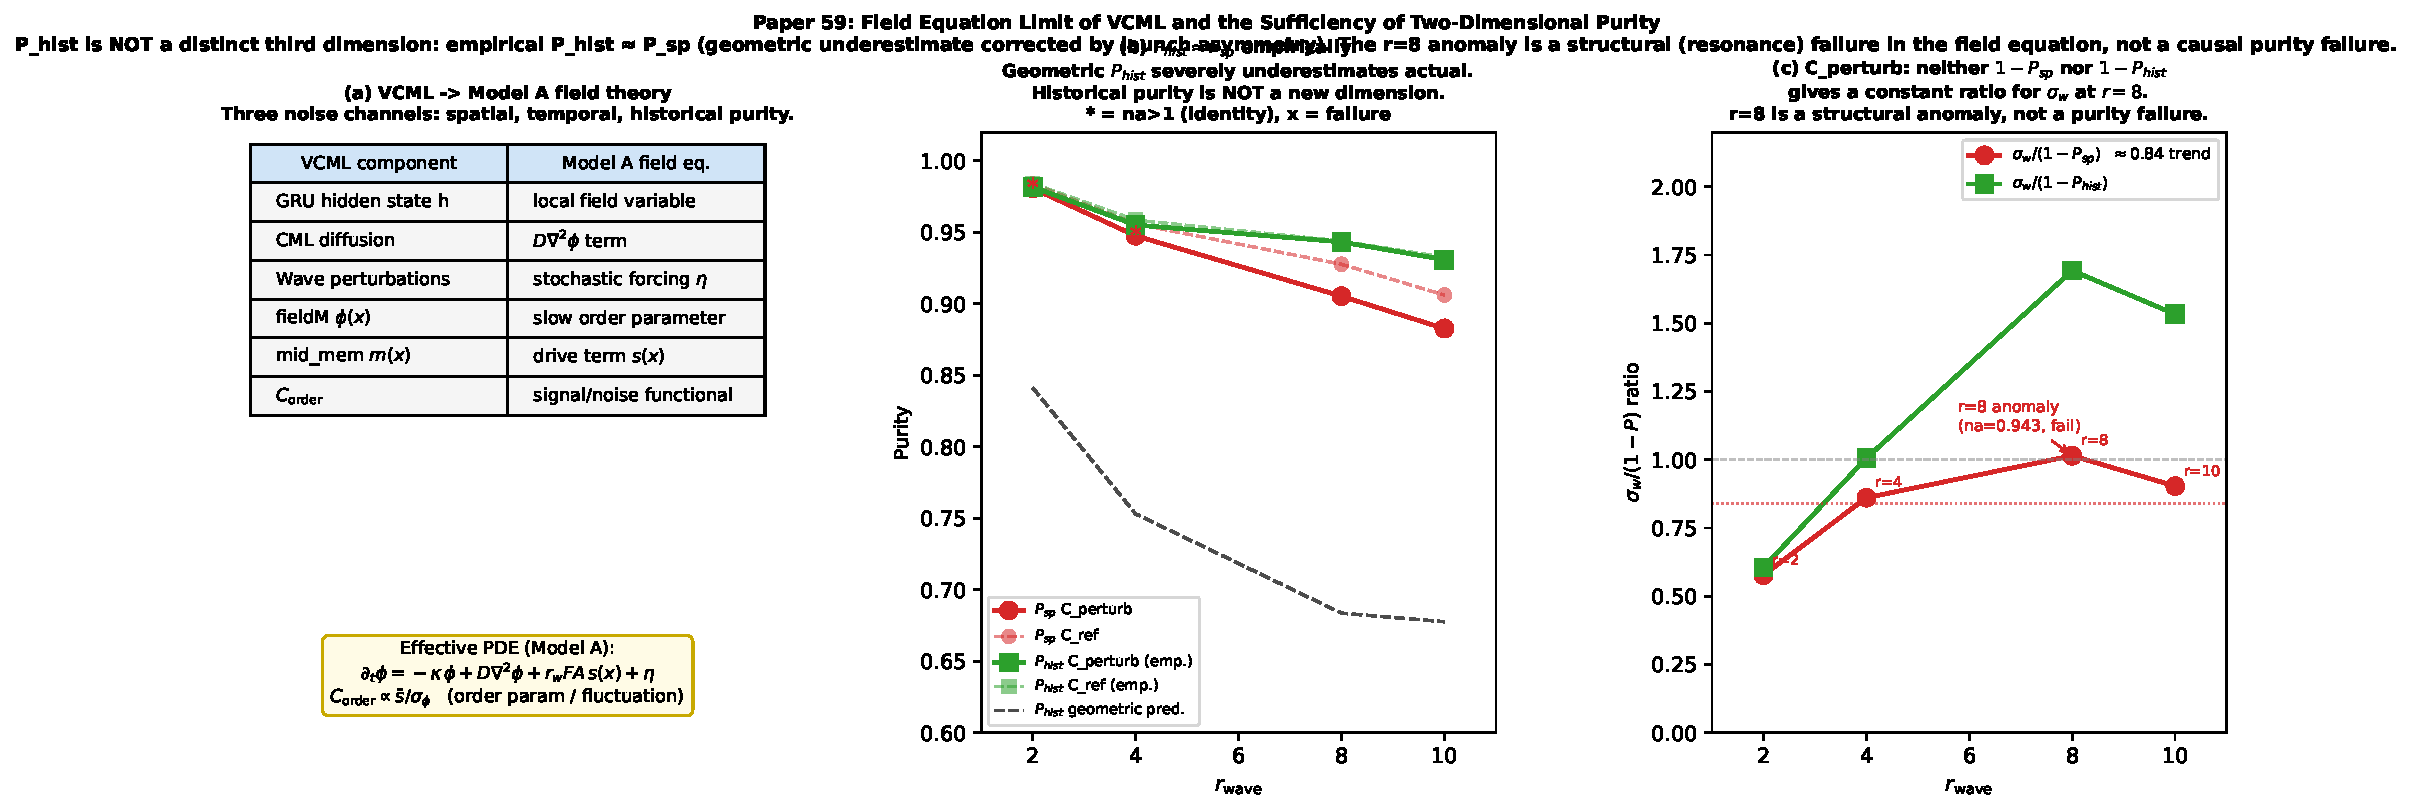
\includegraphics[width=\linewidth]{paper59_figure1.pdf}
  \caption{(a) VCML--Model~A correspondence table and the effective field equation.
    (b) Empirical $\Phist$ vs.\ $\Psp$ for C\_perturb and C\_ref: nearly equal,
    disproving the historical-purity hypothesis.
    Geometric $\Phist$ prediction (dashed) severely underestimates actual purity.
    (c) $\sw/(1-P)$ ratios for C\_perturb with both $P=\Psp$ and $P=\Phist$:
    neither ratio is constant at $r=8$, confirming a structural anomaly
    outside the causal purity framework.}
  \label{fig:main}
\end{figure}

\end{document}
